\chapter{Estado del Arte}
\label{chapter:chapter2}
\section{Fuentes de datos}
Tal y como se ha explicado en la intriducción, durante el desarrollo del proyecto se van a combinar
técnicas de IA Generativa, Redes Neuronales con Aprendizaje por Refuerzo y algoritmos clásicos de 
optimización. Para ello, es necesario tener acceso a distintas fuentes de datos, que se adapten
a cada una de las técnicas que se van a utilizar.\\

De acuerdo con los objetivos propuestos, y el planteamiento general del proyecto, las fuentes de 
datos para este proyecto son las dos siguientes:
\begin{itemize}
    \item \textbf{Electric Vehicle Charging Patterns Dataset}
    \item \textbf{Load Profile Generator}
\end{itemize}

\subsection{Electric Vehicle Charging Patterns Dataset}
\textit{Electric Vehicle Charging Patterns} es un conjunto de datos obtenidoo desde la plataforma
\textit{Kaggle}~\cite{kaggle_ev_charging_patterns}, que contiene información sobre los patrones de 
carga de vehículos eléctricos (EVs) en un entorno urbano. Tal y como lo describe su autor, "otorga 
un análisis exhaustivo de patrones de carga de EVs y comportamiento de los usuarios". El dataset 
incluye 1320 muestras sobre el consumo energético durante la carga, la duración de la carga y 
detalles de cada uno de los vehículos registrados, de entre sus 20 campos.\\
\vfill
\begin{table}[ht]
\begingroup
\centering
\setlength{\tabcolsep}{6pt}
\begin{tabular}{c|l c c c}
 & Modelo & Capacidad (kWh) & SoC Inicial (\%) & SoC Final (\%) \\
\hline
0 & BMW i3 & 108.46 & 29.37 & 86.12 \\
1 & Hyundai Kona & 100.00 & 10.12 & 84.66 \\
2 & Chevy Bolt & 75.00 & 6.85 & 69.92 \\
3 & Hyundai Kona & 50.00 & 83.12 & 99.62 \\
4 & Hyundai Kona & 50.00 & 54.26 & 63.74 \\
\end{tabular}
\caption{Pequeña muestra de los datos del dataset \textit{Electric Vehicle Charging Patterns}.}
\label{tab:ev_charging_patterns_example}
\endgroup
\end{table}

\subsection{Load Profile Generator}
\textit{Load Profile Generator} es una aplicación desarrollada por Noah Pflugradt, de la 
\textit{Bern University of Applied Sciences}~\cite{pflugradt2020loadprofile}
, que genera perfiles de carga sintéticos para un hogar, incluyendo la demanda de energía 
no gestionable, la disponibilidad de carga y los requisitos del vehículo eléctrico. Este 
generador es capaz de crear perfiles de carga sintéticos que simulan el comportamiento 
real de un hogar, lo que permite entrenar y evaluar modelos de IA sin necesidad de datos 
reales.
\begin{figure}[ht]
    \centering
    \includegraphics[width=0.75\textwidth]{images/lpg_logo.png}
    \caption{Logo de LPG. Fuente: \textit{LoadProfileGenerator}~\cite{pflugradt2020loadprofile}.}
    \label{fig:lpg_logo}
\end{figure}

Esta herramienta ha sido instrumental para el desarrollo del proyecto, permitiendo la generación
de consumos completamente realistas, en una amplia variedad de escenarios predefinidos. La 
personalización para la generación de los datos dentro del progama permite generar consumos para
diferentes configuraciones de hogares, variando el número de hijos, su actividad física, la 
distancia al trabajo y muchas más opciones.\\

Además de la variabilidad, en cuanto al análisis de datos se refiere, no sólo facilita el
procesado de los datos, devolviendo los resultados en CSVs (Comma Separated Values) agrupados con 
el consumo global, y también separando por tipos de consumo; sino que el propio programa permite el
ajuste granulado de la resolución temporal interna y externa. De manera que los datos que se han 
generado y se usan en este proyecto, tienen una resolución interna de un minuto, y una resolución 
externa de 15 minutos.

\begin{figure}[ht]
    \centering
    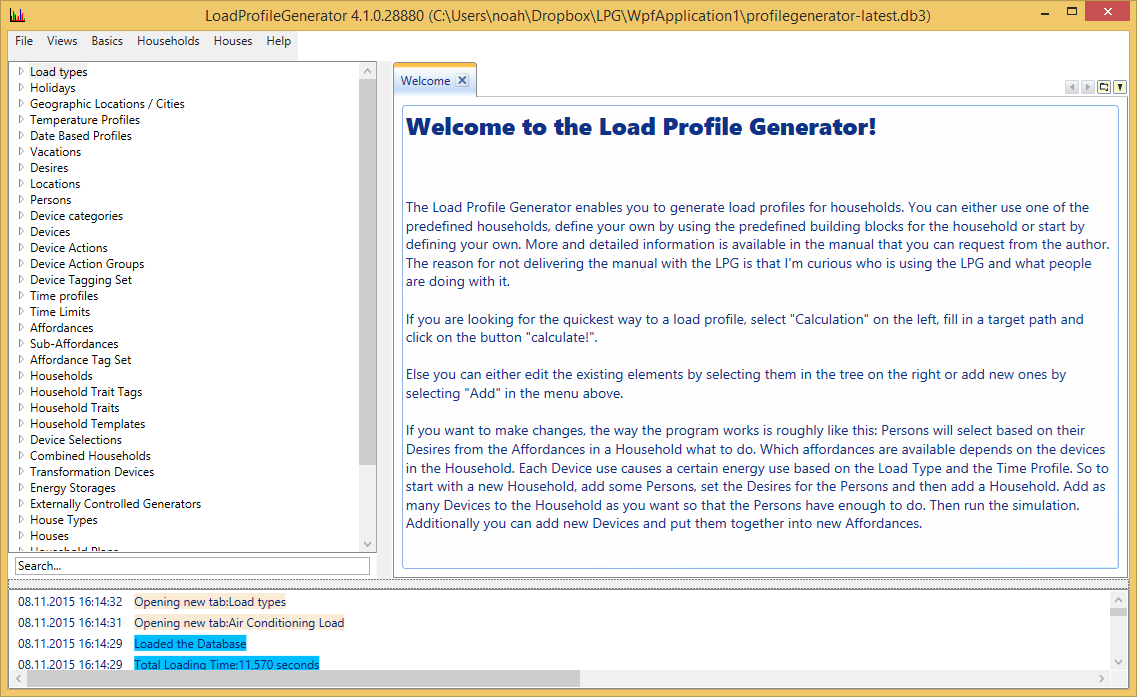
\includegraphics[width=0.7\textwidth]{images/LPG_screenshot.png}
    \caption{Capturas de pantalla de LPG, página principal. 
    Fuente: \textit{LoadProfileGenerator}~\cite{lpg_screenshots_2025}.}
    \label{fig:lpg_screenshot}
\end{figure}
\begin{figure}[ht]
    \centering
    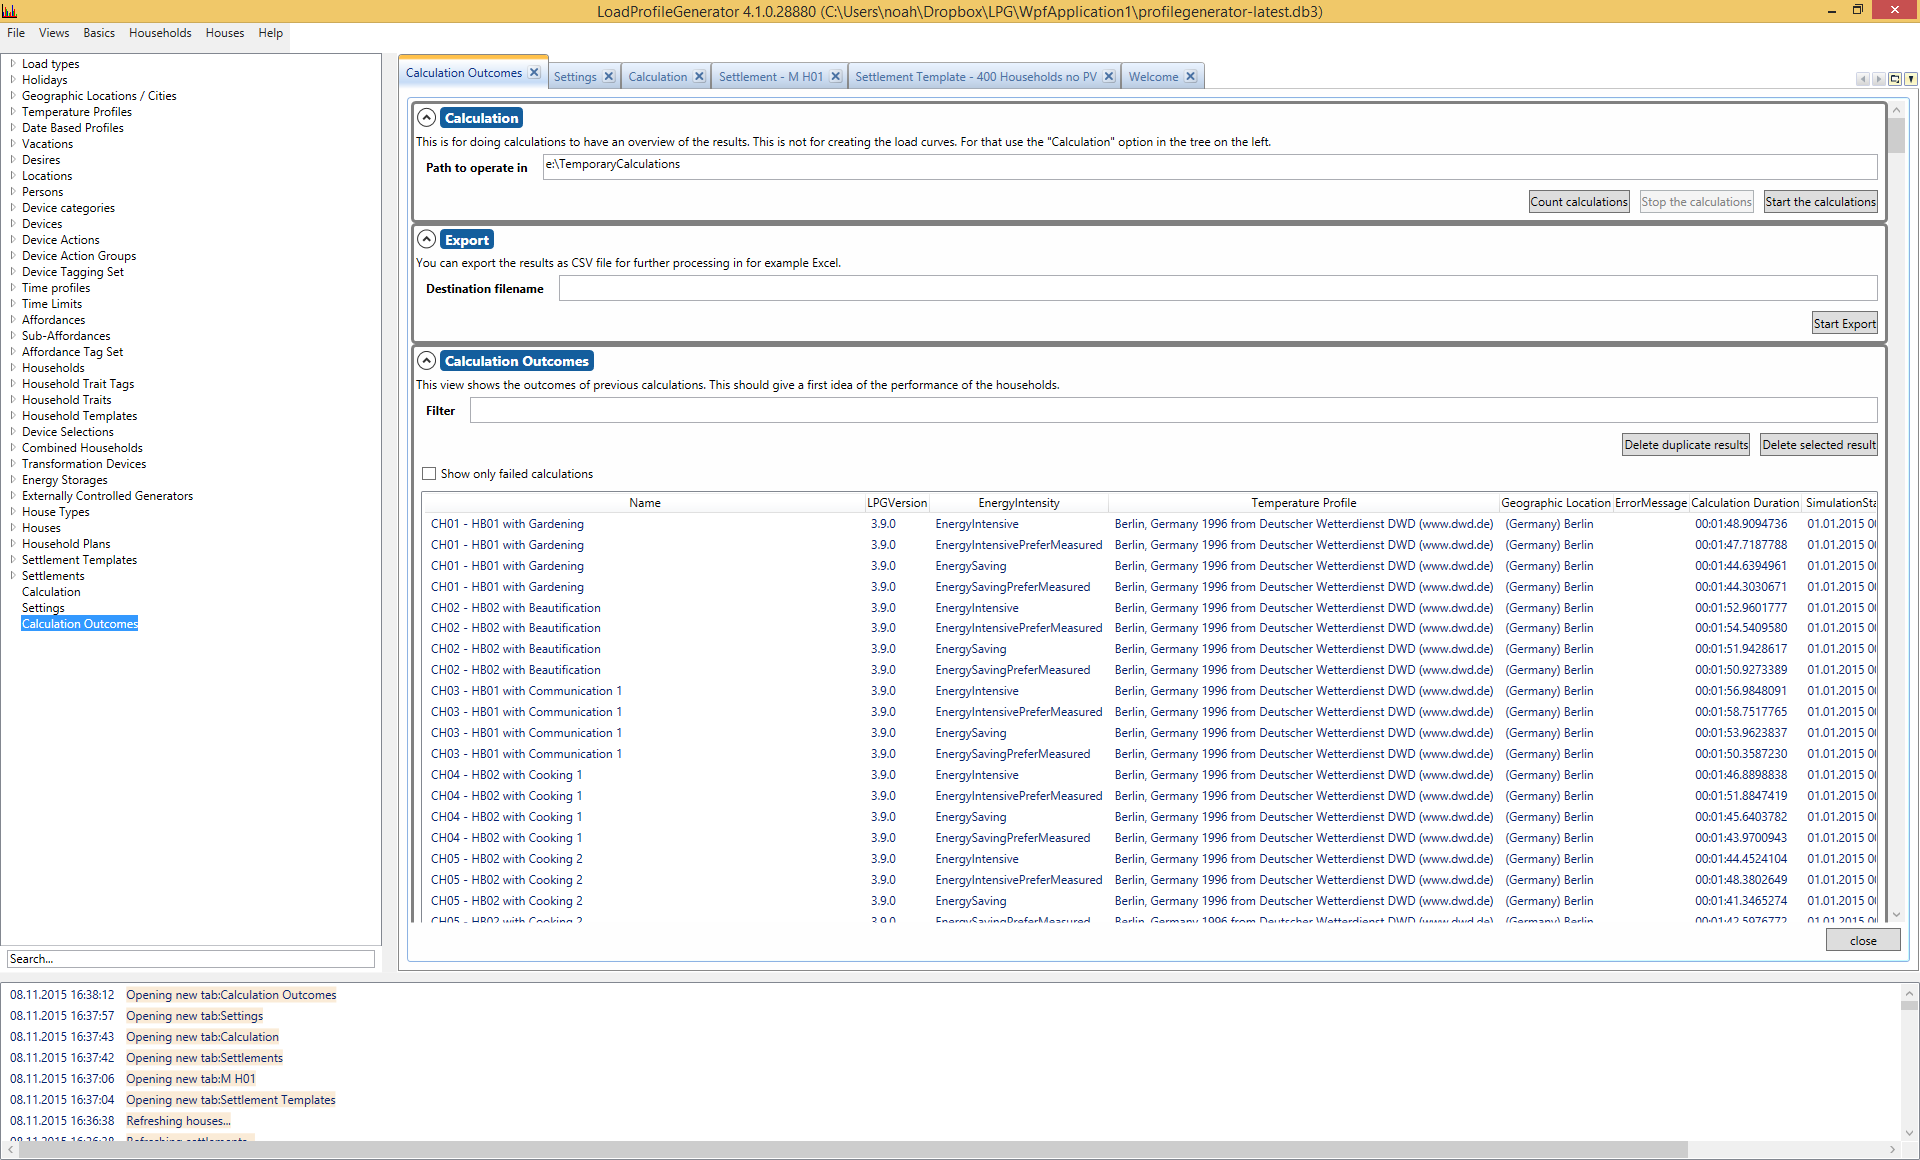
\includegraphics[width=0.7\textwidth]{images/LPG_screenshot_2.png}
    \caption{Capturas de pantalla de LPG, obtención de resultados. 
    Fuente: \textit{LoadProfileGenerator}~\cite{lpg_screenshots_2025}.}
    \label{fig:lpg_screenshot2}
\end{figure}

\section{Optimización Clásica}
La optimización clásica, o programación matemática, es el conjunto de métodos, principios y 
técnicas que se utilizan para encontrar la mejor solución a un problema cuantitativo concreto, 
sujeto a un conjunto de restricciones o condiciones, que limitan el conjunto de soluciones posibles~\cite{wright2025optimization}.
En su forma más básica, la optimización clásica busca maximizar o minimizar una función real, 
referida como función objetivo, resolviendo una serie de ecuaciones y/o desigualdades. Por tanto,
se puede definir la optimización como la elección del mejor elemento dentro de una selección de 
elementos disponibles, sujetos a algún criterio~\cite{wikipedia2025optimizacion}.\\

La optimización clásica se divide en varias categorías, dependiendo de la naturaleza de la función
objetivo y las restricciones. Las categorías más comunes son:
\begin{itemize}
    \item \textbf{Programación Lineal}
    \item \textbf{Programación Entera}
    \item \textbf{Programación No Lineal}
\end{itemize}

\subsection{Programación Lineal}
La programación lineal es un caso concreto del espacio de métodos recogido bajo el término 
\textit{Programación Convexa}. Este concepto se refiere a los programas que resuelven problemas 
en los que la función objetivo es cóncava (maximización) o convexa (minimización). Dentro de este
marco, la programación lineal es el caso particular en el que la función objetivo y las restricciones
son ecuaciones o inecuaciones estrictamente lineales~\cite{wikipedia2025optimizacion}.\\

Geométricamente, puede ser interpretado como si dichas restricciones definieran una figura en el 
espacio euclídeo, y la función objetivo es la dirección en la que se busca maximizar o minimizar el 
valor de la función~\cite{funke2024discreteopt}. Un ejemplo de un problema de programación lineal 
es el siguiente:
\begin{align*}
    \text{Max.} \quad & z = 3x + 2y \\
    \text{Sujeto a} \quad & x + y \leq 4 \\
    & 2x + y \leq 6 \\
    & x \geq 0, \quad y \geq 0
\end{align*}

Aquí, la función objetivo es \(z = 3x_1 + 2x_2\), y las restricciones son claramente lineales. El
objetivo es encontrar los valores de \(x_1\) y \(x_2\) tal que \(z\) sea máxima mientras se cumplen 
las restricciones. La solución óptima se puede encontrar utilizando el método simplex o el método 
de interior-puntos, entre otros algoritmos de optimización lineal~\cite{wikipedia2025optimizacion}.

\subsection{Programación Entera}
Este tipo de programación analiza programas lineales en los que se fuerza que, al menos una de las 
variables, esté forzada a ser un número entero. En este caso particular, la programación entera se
aleja de la programación convexa, ya que la función objetivo y las restricciones no son 
estrictamente lineales, y su resolución suele resultar más compleja que la de un programa lineal 
al uso~\cite{wikipedia2025optimizacion}. La programación entera se divide en dos categorías:
\begin{itemize}
    \item \textbf{Programación Entera \textit{Mixta} (MIP)}: En este caso, algunas variables son enteras y
    otras pueden tomar valores continuos. Este tipo de programación es muy común en problemas de
    optimización combinatoria, donde se busca una solución óptima entre un conjunto discreto de
    opciones, como la asignación de recursos o la planificación de rutas. Hay casos en los que las
    variables pueden tomar valores continuos dentro de un número de opciones discreto, por ejemplo: 
    [0, 0.5, 1] \cite{funke2024discreteopt}.
    \item \textbf{Programación Entera \textit{Pura} (IP)}: En este caso, todas las variables son enteras.
    Este tipo de programación se utiliza en problemas donde todas las decisiones deben ser discretas,
    como la selección de proyectos o la asignación de tareas \cite{funke2024discreteopt}.
\end{itemize}

\subsection{Programación No Lineal}
Como dice su nombre, la programación no lineal es el caso en el que la función objetivo y/o las
restricciones no son lineales \cite{wikipedia2025optimizacion}. Este tipo de programación es más
complejo que la programación lineal, ya que las funciones no lineales pueden tener múltiples
mínimos o máximos locales, lo que dificulta la búsqueda de la solución óptima. Además, la
programación no lineal puede involucrar todo tipo de funciones: cuadráticas, exponenciales, 
logarítmicas o trigonométricas, entre otras \cite{funke2024discreteopt}.

\section{Aprendizaje por Refuerzo (RL)}
Stutton y Barto definen el Aprendizaje por Refuerzo (Reinforcement Learning, RL) como un
"enfoque de aprendizaje automático en el que un agente aprende a tomar decisiones mediante la
interacción con un entorno, recibiendo recompensas o penalizaciones en función de sus acciones".
En otras palabras, RL es aprender qué hacer, asociar situaciones con acciones, para maximizar una
recompensa numérica~\cite{sutton2018reinforcement}.\\

Es importante resaltar la diferencia entre el Aprendizaje Supervisado y el Aprendizaje por Refuerzo. 
En el primer caso, el modelo aprende a partir de un conjunto de datos etiquetados, donde cada 
entrada tiene una salida conocida. En el caso del Aprendizaje por Refuerzo, el modelo aprende a 
partir de su propia experiencia, obtenida tras una serie de interaccioens con el entorno. Por lo 
mismo, el RL es también diferente a lo comúnmente conocido como \textit{Aprendizaje no Supervisado}, 
ya que este grupo de métodos típicamente buscan patrones o estructuras en una colección de datos sin
etiquetar~\cite{sutton2018reinforcement}.\\

Un problema único para los algoritmos de aprendizaje por refuerzo es el equilibrio entre 
exploración y explotación - o \textit{exploration-exploitation trade-off} -. El término exploración
suele hacer referencia a la "curiosidad" del agente por encontrar nuevas y diferentes estrategias,
mientras que explotación se refiere a la tendencia del agente a explotar las estrategias que ya
concoe, y sabe que otorgan resultados positivos. Encontrar un equilibrio balanceado entre estas 
dos características es tremendamente importante para conseguir el aprendizaje posible del agente
\cite{sutton2018reinforcement}.

\subsubsection{Glosario de términos clave en Aprendizaje por Refuerzo}

Tras una breve introducción al Aprendizaje por Refuerzo, es importante definir algunos de los
términos clave que se utilizan en este campo. Estos términos son fundamentales para entender
los conceptos y algoritmos que se desarrollan en el ámbito del RL. A continuación, se presentan
los términos más relevantes y que serán utilizados a lo largo del trabajo:
\cite{wang2022nn_drl}
\begin{itemize}
    \item \textbf{Agente}: Es la parte que toma decisiones y ejecuta acciones dentro del entorno, 
    con el objetivo de maximizar su recompensa acumulada.
    \item \textbf{Acción (A)}: Conjunto de todas las posibles acciones que el agente puede 
    realizar en un estado dado. Una acción concreta se denota habitualmente como \(a\).
    \item \textbf{Factor de descuento (\(\gamma\))}: Parámetro que determina la importancia de las 
    recompensas futuras frente a las inmediatas. Un valor bajo de \(\gamma\) resulta en un agente
    cortoplacista. En caso contrario, el agente tendrá una visión más global y a largo plazo.
    \item \textbf{Estado (S)}: El contexto instantáneo en que se encuentra el agente en cualquier 
    momento.
    \item \textbf{Entorno}: Es el "mundo" en el que opera el agente. Recibe como entrada el estado 
    actual y la acción seleccionada, y devuelve la recompensa obtenida y el nuevo estado resultante.
    \item \textbf{Recompensa (r)}: Retroalimentación que recibe el agente tras ejecutar una acción 
    en un estado determinado. Indica el grado de éxito o fracaso de la acción tomada.
    \item \textbf{Política (\(\pi\))}: Estrategia que sigue el agente para decidir qué acción tomar 
    en cada estado. %Formalmente, es una función que asigna a cada estado la acción que maximiza la recompensa esperada.
    \item \textbf{Valor o Utilidad (V)}: Valor esperado de la recompensa acumulada (a largo plazo y con 
    descuento) que puede obtener el agente desde un estado concreto, siguiendo una política 
    determinada.
    \item \textbf{Valor de acción (Q)}: Valor esperado de la recompensa acumulada (con descuento) 
    que puede obtener el agente al tomar una acción específica en un estado dado, y siguiendo 
    posteriormente una política determinada. Es la función que asigna pares estado-acción a 
    recompensas esperadas.
\end{itemize}

\subsection{Redes Neuronales dentro del RL}
Al final, en un algoritmo de RL, un entorno es una función que transforma una acción en el 
siguiente estado y recompensa, y los agentes son funciones que transforman la función de 
recompensa y el estado en la siguiente acción. Es aquí donde las redes neuronales entran en juego, 
ya que, en esencia, no son más que aproximadores de funciones.\\

Por esta condición de aproximadores de funciones que presentan las redes neuronales, son una 
herramienta excelente cuando el conjunto de acciones y/o de estados es demasiado grande, o no del
todo conocido, siendo este el caso de la inmensa mayoría de los casos de uso en el mundo real.
En estos casos, las redes neuronales pueden aprender a aproximar la función de valor o la política
del agente, permitiendo que el agente tome decisiones informadas basadas en la información
disponible \cite{wang2022nn_drl}.\\

Una RLNN, por ejemplo, puede ser la solución idónea para una IA que aprenda a jugar al ajedrez. El
ajedrez es el juego de estrategia por excelencia, y es tan complejo que no es posible enumerar 
todas las posibles jugadas y resultados. Por tanto, una RLNN puede aprender a jugar al ajedrez a 
través de la experiencia, jugando millones de partidas y ajustando su política de juego en función 
de las recompensas obtenidas al término de cada movimiento o cada partida.

\begin{figure}[ht]
    \centering
    
\includegraphics[width=0.65\textwidth]{images/DeepMind_new_logo.svg.png}
    \caption{Logo de DeepMind. Fuente: DeepMind \cite{deepmind2025website}.}
    \label{fig:deepmind_logo}
\end{figure}

Alpha Zero, la IA desarrollado por Google DeepMind, utiliza una red neuronal con aprendizaje por 
refuerzo, y ha aprendido a jugar al ajedrez, al Go y al shogi con un novel tal, que ha sido capaz
de superar a los mejores jugadores humanos y por supuesto a otros programas de ajedrez, gracias a 
su capacidad para aprender, después de millones de partidas, y adaptarse a diferentes estilos de 
juego \cite{deepmind2017alphazero}.

\subsection{Deep Q-Networks (DQN)}
Una \textit{Deep Q-Network} (DQN) es uno de los algoritmos más potentes y populares en RL, ya que 
hace uso de la combinación de redes neuronales profundas y \textit{Q-Learning}, permitiendo al
agente aprender políticas tremendamente omtimizadas en entornos muy complejos. \cite{dhumne2019dqn}.

\begin{figure}[ht]
    \centering
    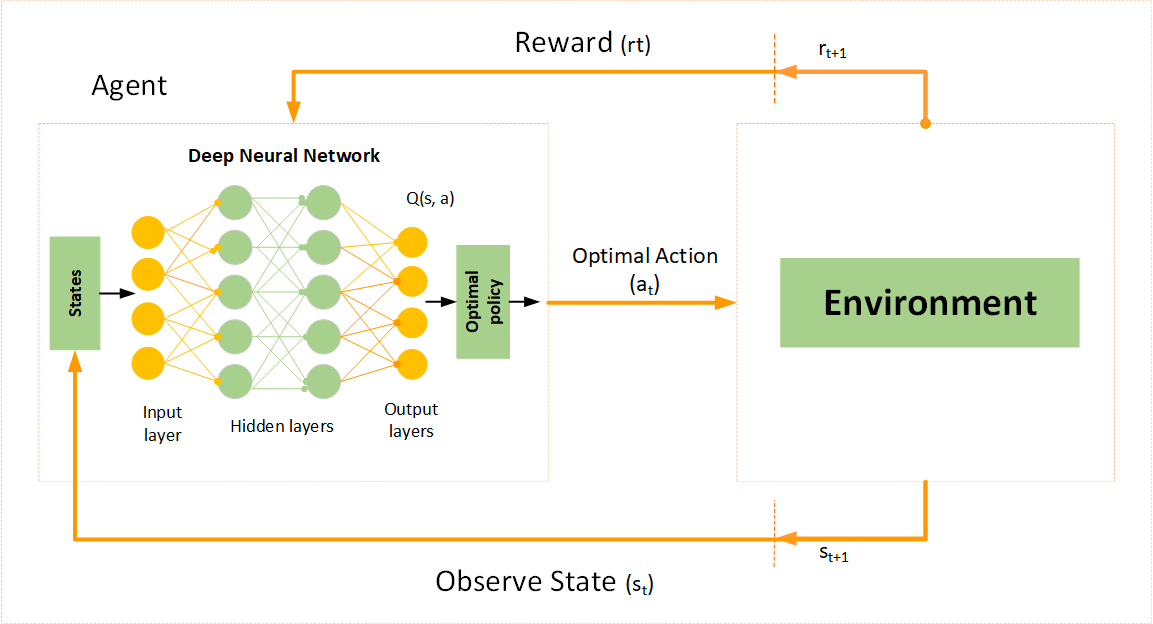
\includegraphics[width=0.9\textwidth]{images/image.png}
    \caption{Arquitectura general de una Deep Q-Network (DQN). Fuente: Deep Q-Learning (DQN)
    \cite{amin2020dqn}.}
    \label{fig:dqn_architecture}
\end{figure}

\textit{Q-Learning} es un algoritmo que enseña a los agentes a comportarse de manera óptima en un 
entorno Markoviano controlado, esto es un entorno en el que la probabilidad de transición entre 
estados depende únicamente del estado actual y la acción tomada, y no de estados anteriores. 
Funciona mejorando iterativamente la evaluación de una acción específica en un estado determinado
\cite{watkins1992qlearning}.

\subsubsection{Funcionamiento de DQN \cite{mnih2013dqn}}
El algoritmo Deep Q-Network (DQN) es una técnica de aprendizaje por refuerzo que utiliza redes 
neuronales para aprender a tomar decisiones. En lugar de trabajar con tablas de valores como el 
Q-learning tradicional, DQN usa una red para aproximar los valores \( Q(s, a) \), que indican lo 
buena que es una acción \( a \) en un estado \( s \).

\begin{itemize}
    \item \textbf{Valor objetivo (Ecuación de Bellman):} Para aprender, DQN compara su predicción 
    con un valor objetivo, calculado usando la ecuación de Bellman:
        \[
        y = r + \gamma \max_{a'} Q(s', a'; \theta^-)
        \]
     donde:
    \begin{itemize}
        \item \( r \) es la recompensa obtenida tras hacer una acción,
        \item \( s' \) es el siguiente estado,
        \item \( \gamma \) es un número entre 0 y 1 que da más o menos importancia a las recompensas 
        futuras,
        \item \( \theta^- \) son los parámetros de una copia de la red (llamada red objetivo).
    \end{itemize}
    Esta actualización sigue el principio de optimalidad de Bellman, que define cómo se calcula el valor óptimo esperado de una acción en un estado.

    \item \textbf{Función de pérdida:} La red aprende minimizando la diferencia entre lo que predice 
    y el valor objetivo:
    \[
    L(\theta) = \mathbb{E}_{(s, a, r, s') \sim D} \left[ \left( y - Q(s, a; \theta) \right)^2 \right]
    \]
    Aquí, \( D \) es un conjunto de experiencias almacenadas (replay buffer), que permite entrenar de 
    forma más estable y variada.

    \item \textbf{Entrenamiento:} Los parámetros \( \theta \) de la red se actualizan usando un 
    algoritmo de optimización (como descenso de gradiente) que intenta reducir el error en las 
    predicciones.

    \item \textbf{Red objetivo:} Para evitar que el entrenamiento sea inestable, DQN usa una segunda 
    red (la red objetivo) que se mantiene fija durante varios pasos y se actualiza solo cada cierto 
    tiempo copiando los valores de la red principal.
\end{itemize}

\subsubsection{Ventajas de DQN \cite{dhumne2019dqn}}
\begin{itemize}
    \item[(+)] El uso de redes neuronales profundas otorga a DQN la capacidad de aprender 
    representaciones abstractas y de alta dimensionalidad, facilitando el aprendizaje en entornos 
    complejos.
    \item[(+)] La utilización de un \textit{replay buffer} permite un entrenamiento más estable y 
    eficiente, ya que el agente puede revisar experiencias pasadas y no depende únicamente de las 
    más recientes.
    \item[(+)] DQN tiene una gran capacidad de generalización, permitiéndole desenvolverse en 
    situaciones no vistas previamente, lo que lo hace muy adecuado para problemas de RL complejos.
\end{itemize}

\subsubsection{Inconvenientes de DQN \cite{dhumne2019dqn}}
\begin{itemize}
    \item[(-)] DQN es sensible a la elección de hiperparámetros, como la tasa de aprendizaje, el 
    factor de descuento, el ratio de exploración y el tamaño del \textit{replay buffer}, lo que 
    puede afectar significativamente su rendimiento.
    \item[(-)] No está diseñado para su uso en línea, siendo más adecuado para entornos 
    \textit{offline}.
    \item[(-)] La actualización de \textit{Q-learning} implementada en DQN puede ser propensa a la 
    sobreestimación de los valores \( Q \).
\end{itemize}

\subsection{Long Short-Term Memory (LSTM)}
Las redes \textit{Long Short-Term Memory} (LSTM) son una arquitectura de redes neuronales 
recurrentes (RNNs) diseñada para gestionar información secuencial - como las series temporales - de 
forma más eficaz. A diferencia de las RNN simples, que utilizan un único vector oculto para 
propagar información, las LSTM incorporan una estructura interna más compleja que les permite 
mantener información relevante durante más tiempo y decidir qué conservar y qué 
olvidar~\cite{bulling2024rnn}.

\begin{figure}[ht]
    \centering
    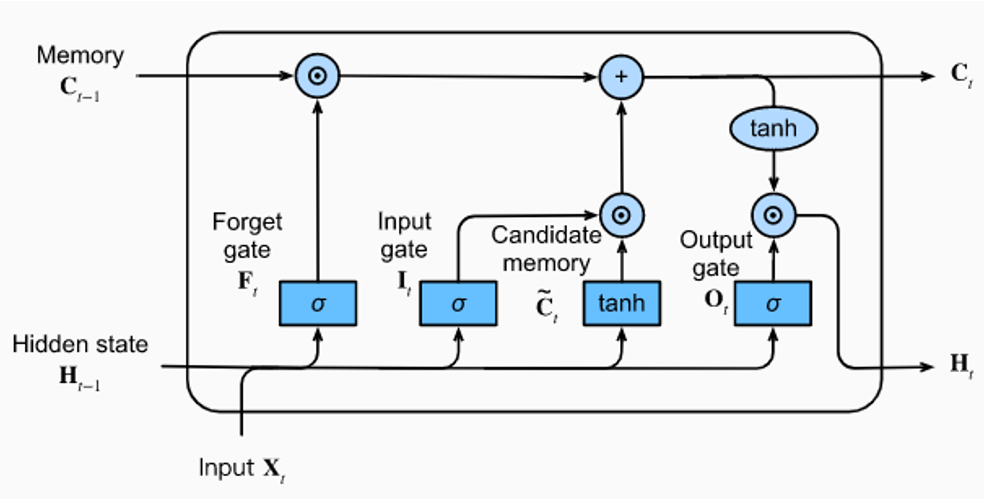
\includegraphics[width=0.8\textwidth]{images/LSTM_diagram.png}
    \caption{Diagrama LSTM. Fuente: \textit{An Intuitive Explanation of LSTM}~\cite{calzone2020lstm}.}
    \label{fig:lstm_diagram}
\end{figure}

Internamente, una LSTM introduce tres puertas: la \textit{puerta de entrada}, la 
\textit{puerta de olvido} y la \textit{puerta de salida}. Estas puertas actúan como filtros que 
controlan el flujo de información a lo largo del tiempo:
\begin{itemize}
    \item La puerta de entrada determina qué parte de la información nueva debe almacenarse.
    \item La puerta de olvido decide qué parte del contenido anterior debe descartarse.
    \item La puerta de salida regula qué información del estado interno se transmite a la 
    siguiente capa o paso de tiempo.
\end{itemize}

Gracias a esta estructura, las LSTM son especialmente útiles para tareas donde es importante 
tener en cuenta el contexto anterior, como el procesamiento de lenguaje natural, la clasificación 
de secuencias o la predicción de series temporales. La capacidad de decidir dinámicamente qué 
recordar y qué olvidar convierte a las LSTM en una herramienta eficaz para trabajar con 
dependencias temporales prolongadas \cite{calzone2020lstm}. Estas propiedades hacen que las LSTM 
sean más robustas para modelar dependencias a largo plazo en secuencias, en comparación con las RNN 
simples.

\section{Técnicas de IA Generativa}
A lo largo de esta sección, se tratará de explicar y exponer las principales técnicas usadas en el
mundo de la inteligencia artificial generativa, que pueden trasladarse de manera práctica al 
sector eléctrico. Las cuatro técnicas que tratar son:

\begin{itemize}
    \item \textbf{Generative Adversarial Networks (GANs)}
    \item \textbf{Variational Autoencoders (VAEs)}
    \item \textbf{Modelos de difusión}
    \item \textbf{Modelos fundacionales}
\end{itemize}

\subsection{Generative Adversarial Networks (GANs)}
Esta primera técnica, emplea aprendizaje no supervisado con dos redes neuronales contrapuestas. 
Éstas, son entrenadas de manera que compiten entre sí, en un proceso similar a un juego de “suma 
cero”.\\

Durante el entrenamiento, una de las dos redes, la red A, genera candidatos para ser evaluados por 
la red B. Normalmente, la red A se entrena para que genere candidatos y estímulos siguiendo una 
determinada distribución o reglas, mientras que la red B pretende discriminar y diferenciar casos 
originales de casos generados artificialmente.\\

Con este planteamiento, el objetivo es complicarle la tarea a la red B, consiguiendo que el output 
de la red A sea tan similar al original, que dificulte la diferenciación. \cite{xiao2022gan}.

\begin{table}[H]
\centering
\begin{tabularx}{\textwidth}{X|X}
    \textbf{Fortalezas} & \textbf{Debilidades} \\ \hline
    Generación de imágenes & Entrenamiento complejo \\ 
    Reescalado & Inestabilidad y ``mode collapse'' \\
    Multimodalidad & \\ 
    Gran versatilidad & \\ 
\end{tabularx}
\caption{Fortalezas y debilidades de las GANs}
\end{table}

\subsection{Variational Autoencoders (VAEs)}
El segundo tipo de modelo generativo, los Autocodificadores Variacionales, son modelos que aprenden 
de sus datos como una representación comprimida de los mismos, asignados a una distribución 
probabilística, que luego se usará para generar variaciones de estos. Es decir, los VAE aprenden a 
identificar y extraer las características más relevantes de los datos con los que son entrenados. \cite{moradzadeh2022vae}.\\

\begin{table}[H]
\centering
\begin{tabularx}{\textwidth}{X|X}
    \textbf{Fortalezas} & \textbf{Debilidades} \\ \hline
    Extracción componentes principales & Entrenamiento delicado \\ 
    Compresión de datos & Ejemplos borrosos \\ 
    Generar variaciones de datos entrenamiento & Interpretación de expertos \\ 
\end{tabularx}
\caption{Fortalezas y debilidades de los VAEs}
\end{table}

\subsection{Modelos de difusión}
En tercer lugar, los modelos de difusión son una técnica de generación de datos muy utilizada para 
imágenes, que funciona de forma diferente a otros enfoques expuestos anteriormente, como las GANs.\\

En lugar de un sistema entre dos redes, los modelos de difusión utilizan un proceso gradual de 
adición y eliminación de ruido. El proceso de entrenamiento consiste en añadir ruido de forma 
progresiva a los datos originales, hasta que se vuelven irreconocibles para luego revertir este 
proceso, eliminando el ruido paso a paso, hasta recuperar una versión clara de los datos. Esto 
permite que el modelo pueda generar nuevas imágenes, u otro formato de datos, comenzando desde 
ruido aleatorio, porque ha aprendido a reconstruir datos realistas a partir de ruido. \cite{weng2021diffusion}.

\begin{table}[H]
\centering
\begin{tabularx}{\textwidth}{X|X}
    \textbf{Fortalezas} & \textbf{Debilidades} \\ \hline
    Generación desde ruido aleatorio & Mayor tiempo de computación \\ 
    Alto nivel de detalle & Mayor coste computacional \\ 
    Multimodalidad & Poca versatilidad \\ 
\end{tabularx}
\caption{Fortalezas y debilidades de los Modelos de Difusión}
\end{table}

\subsection{Modelos Fundacionales}
Finalmente, los modelos fundacionales son la punta de lanza de la IA Generativa. Son un tipo de 
modelo de Deep Learning, que ha sido entrenado con una vastísima y muy diversa cantidad de datos 
desestructurados y sin etiquetar. Lo que los hace destacar es su capacidad de aprendizaje 
generalizado, que les permite transferir sus conocimientos a diversas tareas sin necesidad de ser 
específicamente entrenados para ellas. Estos modelos, que pueden generar o comprender texto, 
imágenes, audio, entre otros formatos, resultan muy útiles en aplicaciones que requieran una 
entendimiento profundo del contexto o la creación de nuevos contenidos en distintos formatos. \cite{umay2024llms}.\\

Entre ellos, los Modelos de Lenguaje Extensos (LLMs), como GPT o BERT, permiten generar y 
comprender texto de manera eficiente. Por su parte, los Modelos de Lenguaje Pequeños (SLMs) ofrecen 
soluciones más ligeras y específicas. 

\begin{table}[H]
\centering
\begin{tabularx}{\textwidth}{X|X}
    \textbf{Fortalezas} & \textbf{Debilidades} \\ \hline
    Versatilidad sin conocimiento específico & Necesidad de gran cantidad de datos \\ 
    Multimodalidad & Posibilidad de sesgos \\
    Eficiencia & Posibilidad información desactualizada \\ 
    Prolificidad & Conocimiento limitado \\ 
\end{tabularx}
\caption{Fortalezas y debilidades de los Modelos Fundacionales}
\end{table}

\subsection{Aplicaciones en el sector eléctrico}

A continuación, se muestra una comparativa con las distintas aplicaciones y servicios de las 
anteriores técnicas en el sector eléctrico, así como qué técnicas serían necesarias para cada 
servicio, el riesgo, y qué mejorarían:

% Definir colores
\definecolor{risk1}{rgb}{0.9, 0.93, 0.97}
\definecolor{risk2}{rgb}{0.8, 0.88, 0.97}
\definecolor{risk3}{rgb}{0.7, 0.82, 0.95}
\definecolor{risk4}{rgb}{0.6, 0.76, 0.92}
\definecolor{risk5}{rgb}{0.4, 0.6, 0.8}

\newcommand{\cmark}{\ding{51}} % Símbolo de check ✔



% Nueva tabla con ajuste de anchos para aprovechar el espacio horizontal y eliminar huecos en blanco
\begin{table}[H]
\scriptsize
\centering
\caption{Clasificación de las distintas aplicaciones. Siendo los números en la segunda columna cada 
una de las técnicas por orden: (1) GANs, (2) VAEs, (3) Modelos de difusión, (4) Modelos fundacionales.}
\label{tab:comparativa_aplicaciones}
\renewcommand{\arraystretch}{1.5} % Aumentar el espacio entre filas
\setlength{\tabcolsep}{3.5pt}
\begin{tabularx}{\textwidth}{>{\raggedright\arraybackslash}p{3.5cm} c >{\centering\arraybackslash}p{1.1cm} 
>{\centering\arraybackslash}p{1.7cm} 
>{\centering\arraybackslash}p{1.7cm} 
>{\centering\arraybackslash}p{1.7cm} 
>{\centering\arraybackslash}p{2.2cm}}
%\toprule
\textbf{Aplicación} & \textbf{Técnicas} & \textbf{Riesgo} & \multicolumn{4}{c}{\textbf{Mejora}} \\
\cmidrule(lr){4-7}
& & & \textit{Temporal} & \textit{Económica} & \textit{Mantenimiento} & \textit{Cualitativa} \\
%\midrule
Detección de anomalías & 1,3 & \cellcolor{risk1} & \cmark & \cmark & \cmark & \cmark \\
Creación de imágenes & 1,3,4 & \cellcolor{risk2} & \cmark & \cmark & & \cmark \\
Análisis de imágenes & 1,2,4 & \cellcolor{risk2} & \cmark & \cmark & \cmark & \cmark \\
Generación escenarios consumo & 1,2 & \cellcolor{risk3} & \cmark & \cmark & & \cmark \\
Predicciones (Demanda y Prod.) & 1,2,4 & \cellcolor{risk3} & \cmark & \cmark & & \cmark \\
Análisis de mercado & 2,4 & \cellcolor{risk4} & \cmark & \cmark & & \cmark \\
Estimación de estados & 1,2 & \cellcolor{risk5} & \cmark & \cmark & \cmark & \cmark \\
Interfaz interactiva & 4 & \cellcolor{risk2} & \cmark & & & \cmark \\
%\bottomrule
\end{tabularx}
\end{table}

El riesgo se refiere a la seguridad de las aplicaciones, y cómo de seguro es realizar una
inversión en cada una de ellas. Con ello, se tiene en cuenta el nivel y oportunidades de
desarrollo en cada uno de los campos, la volatilidad de estos. Por tanto, un proyecto de
sencilla aplicación con oportunidad de desarrollo va a ser más “seguro” que otra alternativa
que encuentre mayor dificultad de implementación o desarrollo.\\

Los tipos de mejora a los que se hace referencia describen los campos en los que cada
aplicación puede ofrecer beneficios. De esta manera, la mejora temporal se refiere a que la
aplicación ofrece mayor eficiencia en el tiempo que la herramienta o proceso que estaría
reemplazando. Del mismo modo, la mejora económica indica que dicha aplicación incurre
en menor coste, bien sea coste fijo, variable o de instalación, que las posibles alternativas.\\

Las aplicaciones marcadas positivamente en la casilla de mantenimiento quieren decir que
ofrecen soluciones con mejores resultados para procesos de mantenimiento. Finalmente, la
mejora cualitativa indica que las ventajas que plantea la aplicación son transversales, y se
ven reflejadas directamente en la calidad de experiencia para el usuario.